\section{Intel x86 and ARM}
\begin{framedremark}
This material is not on the final 
\end{framedremark}

\paragraph{Intel Processors}%
\label{par:Intel Processors}
\begin{table}[h]
\centering
\begin{tabular}{|l|c|c|c|p{7cm}|}
\hline
\textbf{Processor} & \textbf{Date} & \textbf{f (MHz)} & \textbf{Trans.} & \textbf{Features} \\
\hline
4004 & 4/71 & 0.108 & 2.3k & First $\mu$P \\
8008 & 4/72 & 0.108 & 3.5k & First 8-bit $\mu$P \\
8080 & 4/74 & 2 & 6k & Popular 8-bit \\
8086 & 6/78 & 5--10 & 29k & First 16-bit $\mu$P; 20-bit addressing \\
8088 & 6/79 & 5--8 & 29k & Simpler; IBM PC \\
80286 & 2/82 & 8--12 & 134k & Protected mode; 24-bit addressing \\
80386 & 10/85 & 16--33 & 275k & 32-bit (x86) \\
80486 & 4/89 & 25--100 & 1.2M & Pipelined (5-stage); cache \\
Pentium & 3/93 & 60--233 & 3.1M & Superscalar; dual pipeline \\
Pentium Pro & 3/95 & 150--200 & 5.5M & Out-of-order; L2 cache \\
Pentium II & 5/97 & 233--400 & 7.5M & MMX (SIMD instructions) \\
Pentium III & 3/99 & 450--1400 & 9.5--28M & SSE (incl.\ SIMD-FP); 10-stage pipeline \\
Pentium 4 & 12/00 & 1300--2200 & 42M & SSE2 (128-bit); TC; 20-stage pipeline \\
NetBurst & 04/04 & 800--3800 & 376M & 64-bit (x86-64); SSE3; HT; 31-stage pipeline \\
Core & 06/06 & up to 3300 & 105M & SSSE3; SSE4; 12--14-stage pipeline \\
Nehalem & 11/08 & up to 3600 & 731M & 20--24-stage pipeline \\
Sandy Bridge & 01/11 & up to 4000 & -- & AVX (256-bit, 3-op); 14--19-stage pipeline \\
Haswell & 06/13 & up to 4400 & -- & AVX2 \\
Skylake & 08/15 & up to 3700 & -- & AVX-512 (512-bit) \\
\hline
\end{tabular}
\caption{Evolution of Intel Microprocessors}
\end{table}
As we have seen before the growth of the number of transistors for processors is exponential:
\begin{center}
\includegraphics[scale=0.18]{screenshots/2025-12-16.png}
\end{center}
Remember that we want to stay at the same price for our processors \textrightarrow we add more transistors in our processors. This is the reason for the growth of transistors. But this number of transistors may not be that useful.

\definecolor{lightgray}{gray}{0.93}

\begin{table}[ht]
\centering
\small
\rowcolors{2}{lightgray}{white}
\resizebox{\textwidth}{!}{%
\begin{tabular}{l|ccccccc}
\hline
Processor &
Intel 1-core Xeon &
AMD 1-core Opteron 854 &
Intel 2-core Xeon X5270 &
AMD 2-core Opteron 8224SE &
Intel 4-core Xeon X7350 &
AMD 4-core Opteron 8360SE &
Intel 6-core Xeon X7460 \\
\hline
\hline
Bit-width & 32/64 & 32/64 & 32/64 & 32/64 & 32/64 & 32/64 & 32/64 \\
Cores/chip × threads/core & $1\times2$ & $1\times1$ & $2\times1$ & $2\times1$ & $4\times1$ & $4\times1$ & $6\times1$ \\
Clock rate & 3.80 GHz & 2.80 GHz & 3.50 GHz & 3.20 GHz & 2.93 GHz & 2.50 GHz & 2.67 GHz \\
Cache L1-L2-L3 &
12K/16K -- 2M &
64K/64K -- 1M &
$2\times32$K/$32$K -- 6M &
$2\times64$K/$64$K -- $2\times1$M &
$4\times32$K/$32$K -- $2\times4$M &
$4\times64$K/$64$K -- $4\times512$K &
$6\times32$K/$32$K -- $3\times3$M \\
Execution rate/core & 3 instr. & 3 instr. & 1 complex + 3 simple & 3 instr. & 1 complex + 3 simple & 3 instr. & 1 complex + 3 simple \\
Pipeline stages & 31 & 12 int / 17 fp & 14 & 12 int / 17 fp & 14 & 12 int / 17 fp & 14 \\
Out-of-order & 126 & 72 & 96 & 72 & 96 & 72 & 96 \\
Memory bus & 800 MHz & 6.4 GB/s & 1333 MHz & 10.6 GB/s & 1066 MHz & 10.6 GB/s & 1064 MHz \\
Package & LGA-775 & uPGA 940 & LGA-771 & LGA-1207 & LGA-771 & LGA-1207 & LGA-771 \\
IC process & 90 nm & 90 nm & 45 nm & 90 nm & 65 nm & 65 nm & 45 nm \\
Die size & 109 mm$^2$ & 106 mm$^2$ & 107 mm$^2$ & 227 mm$^2$ & $2\times143$ mm$^2$ & 283 mm$^2$ & 503 mm$^2$ \\
Transistors & 169 M & 120 M & 410 M & 233 M & $2\times291$ M & 463 M & 1900 M \\
List price & \$903 & \$1,514 & \$1,172 & \$2,149 & \$2,301 & \$2,149 & \$2,729 \\
Availability & 3Q05 & 3Q05 & 3Q08 & 3Q07 & 3Q07 & 2Q08 & 4Q08 \\
Scalability & 1--2 chips & 2--4 chips & 1--2 chips & 1--4 chips & 1--4 chips & 2--4 chips & 1--4 chips \\
SPECfp2006 & 11.4 / 11.7 & 11.2 / 12.1 & 26.5 / 25.5 & 14.1 / 14.2 & 21.7 / 18.9 & 14.4 / 18.5 & 22.0 / 22.3 \\
SPECfp2006\_rate & 20.9 / 18.8 & 41.4 / 45.6 & 84.9 / 57.7 & 105 / 96.7 & 184 / 108 & 170 / 156 & 274 / 142 \\
x86 codename & Irwindale & Athens & Wolfdale & Santa Rosa & Tigerton & Barcelona & Dunnington \\
Microarchitecture & NetBurst & K8 & Core & K8 & Core & K10 & Core \\
\hline
\end{tabular}}
\end{table}


\begin{table}[ht]
\centering
\small
\rowcolors{2}{lightgray}{white}
\resizebox{\textwidth}{!}{%
\begin{tabular}{l|ccccccc}
\hline
Processor &
Intel Itanium 2 9050 &
Intel Itanium 2 9150M &
IBM POWER5+ &
IBM POWER6 &
Fujitsu SPARC64 VI &
Fujitsu SPARC64 VII &
Sun UltraSPARC T2+ \\
\hline
Bit-width & 64 & 64 & 64 & 64 & 64 & 64 & 64 \\
Cores/chip × threads/core & $2\times2$ & $2\times2$ & $2\times2$ & $2\times2$ & $2\times2$ & $4\times2$ & $8\times8$ \\
Clock rate & 1.60 GHz & 1.67 GHz & 2.20 GHz & 5.00 GHz & 2.40 GHz & 2.52 GHz & 1.40 GHz \\
Cache L1-L2-L3 &
$2\times16$K/$16$K -- 12M(on) &
$2\times16$K/$16$K -- 12M(on) &
$2\times64$K/$32$K -- 1.92M(off) &
$2\times64$K/$64$K -- 32M(off) &
$2\times128$K/$128$K -- 6M &
$4\times64$K/$64$K -- 6M &
$8\times8$K/$16$K -- 4M \\
Execution rate/core & 6 issue & 6 issue & 5 issue & 7 issue & 4 issue & 4 issue & 16 issue \\
Pipeline stages & 8 & 8 & 15 & 13 & 15 & 15 & 8 int / 12 fp \\
Out-of-order & None & None & 200 & Limited & 64 & 64 & None \\
Memory bus & 8.5 GB/s & 10.6 GB/s & 12.8 GB/s & 75 GB/s & 8 GB/s & 8 GB/s & 42.7 GB/s \\
Package & mPGA-700 & mPGA-700 & MCM-5370 pins & N/A & 412 I/O pins & 412 I/O pins & 1831 pins \\
IC process & 90 nm & 90 nm & 90 nm & 65 nm & 90 nm & 65 nm & 65 nm \\
Die size & 596 mm$^2$ & 596 mm$^2$ & 245 mm$^2$ & 341 mm$^2$ & 421 mm$^2$ & 400 mm$^2$ & 342 mm$^2$ \\
Transistors & 1.72 B & 1.72 B & 276 M & 790 M & 540 M & 600 M & 503 M \\
List price & \$3,692 & \$3,692 & N/A & N/A & N/A & N/A & N/A \\
Availability & 3Q06 & 4Q07 & 4Q05 & 2Q08 & 2Q07 & 3Q08 & 2Q08 \\
Scalability & 1--64 chips & 8--128 chips & 1--32 chips & 2--32 chips & 4--64 chips & 4--64 chips & 2 chips \\
SPECfp2006 & 14.5 / 17.3 & N/A & 10.5 / 12.9 & 15.8 / 20.1 & 9.7 / 21.7 & 10.5 / 25.0 & N/A \\
SPECfp2006\_rate & 1534 / 1671 & 2893 / N/A & 197 / 229 & 1837 / 1822 & 1111 / 1160 & 2088 / 1861 & 142 / 111 \\
Architecture status & Inactive & Active & Inactive & Active & Inactive & Active & Active \\
\hline
\end{tabular}}
\end{table}

So here the Intel Itanium 2 9050 and Intel Itanium 9150M are the only LVIW processors here. As we can see in the Out of Order line there is \textit{none} in both of them.
\begin{framedremark}
As we can see there is 1.72 \important{billion} transistors for those two processors. But didn't we say that we needed less transistors for them? Yes in theory, but only if you are focusing on one type of program. This cannot work for general purpose program.
\end{framedremark}

\begin{parag}{Legacy x86 Features}
    \begin{itemize}
		\item Very \important{small number of registers}, partly dedicated or \important{specialised}
		\item Natively 16-bit, extended to 32 in successive steps requiring backward compatibility (e.g., 3 modes for address generation)
		\item \important{Highly variable instruction length} and encoding (1 to 17 bytes in original x86, prefixes, postfixes, etc.)
		\item \important{CISC} instruction set
    \end{itemize}
    
\end{parag}


\begin{parag}{Registers}
    There is a very small number of general purpose registers (approx. 4 integer plus 8 FP -- not shown, versus 32+32 typ. RISC)
	\begin{center}
	\includegraphics[scale=0.3]{screenshots/2025-12-16_2.png}
	\end{center}
	\begin{center}
	\includegraphics[scale=0.3]{screenshots/2025-12-16_3.png}
	\end{center}
	\begin{itemize}
		\item small number of registers makes spilling more frequent
		\item Advanced compiler technique (e.g., loop unrolling) increase registers pressure
		\item Partial specialization of the registers makes \important{effective compiler use difficult}
	\end{itemize}
	
\end{parag}

\begin{parag}{Memory Address}
	You can also see the history of the memory. First we need a physical address that is more than 16 bits (our memory is greater that $2^{16}$) However our architecture at that time is only at 16 bits. We need another register in order for have access to the address.\\
	This is the real mode (8086)
    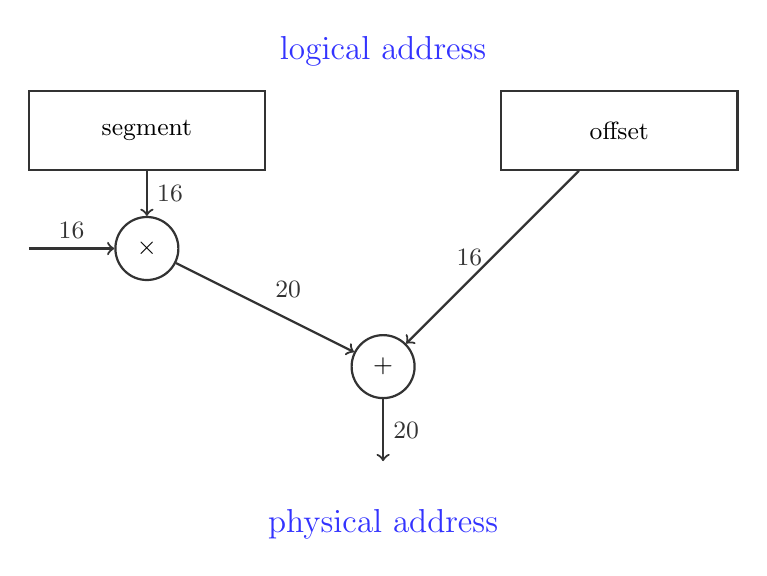
\begin{tikzpicture}[
    font=\small,
    box/.style={draw=black!80, thick, rectangle, minimum width=3cm, minimum height=1cm},
    circ/.style={draw=black!80, thick, circle, minimum size=8mm},
    arrow/.style={->, thick, black!80}
]

% Titles
\node[font=\large, blue!80] at (0,4) {logical address};

% Boxes
\node[box] (segment) at (-3,3) {segment};
\node[box] (offset)  at ( 3,3) {offset};

% Operators
\node[circ] (mul) at (-3,1.5) {$\times$};
\node[circ] (add) at ( 0,0) {$+$};

% Physical address
\node[font=\large, blue!80] at (0,-2) {physical address};

% Arrows
\draw[arrow] (segment) -- node[right] {16} (mul);
\draw[arrow] (mul) -- node[above right] {20} (add);
\draw[arrow] (offset) -- node[left] {16} (add);
\draw[arrow] (add) -- node[right] {20} (0,-1.2);

% Extra input to multiplier (shift left by 4)
\draw[arrow] (-4.5,1.5) -- node[above] {16} (mul);

\end{tikzpicture}
Now if we take a look at the protected mode (80286), now we have a sort of multiprogramming.


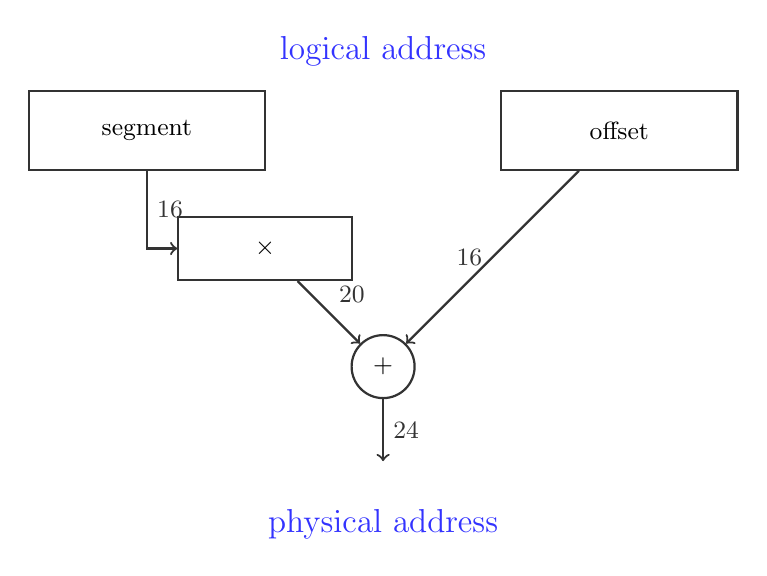
\begin{tikzpicture}[
    font=\small,
    box/.style={draw=black!80, thick, rectangle, minimum width=3cm, minimum height=1cm},
    opbox/.style={draw=black!80, thick, rectangle, minimum width=2.2cm, minimum height=0.8cm},
    circ/.style={draw=black!80, thick, circle, minimum size=8mm},
    arrow/.style={->, thick, black!80}
]

% Title
\node[font=\large, blue!80] at (0,4) {logical address};

% Boxes
\node[box] (segment) at (-3,3) {segment};
\node[box] (offset)  at ( 3,3) {offset};

% Operators
\node[opbox] (mul) at (-1.5,1.5) {$\times$};
\node[circ]  (add) at ( 0,0) {$+$};

% Physical address
\node[font=\large, blue!80] at (0,-2) {physical address};

% Arrows
\draw[arrow] (segment) -- node[right] {16} (-3, 1.5) -- (mul);
\draw[arrow] (mul) -- node[above right] {20} (add);
\draw[arrow] (offset) -- node[left] {16} (add);
\draw[arrow] (add) -- node[right] {24} (0,-1.2);


\end{tikzpicture}

Now if we go even later in the protected mode (80386, 80486, Plentium). we need now to have a bit of multiprogramming right?
\begin{center}
    

\begin{tikzpicture}[
    font=\small,
    box/.style={draw=black!80, very thick, rectangle, minimum width=3.8cm, minimum height=1.2cm},
    mem/.style={draw=black!80, very thick, rectangle, minimum width=3.2cm, minimum height=1cm},
    op/.style={draw=black!80, very thick, circle, minimum size=8mm},
    arrow/.style={->, thick},
    dashedbox/.style={draw=red, dashed, thick, rounded corners, inner sep=8pt}
]

%================ TOP: segmentation =====================

\node[box] (segment) at (-4,5) {segment};
\node[box] (offset)  at ( 4,5) {offset};

\node[mem] (segdesc) at (-1.5,3.6) {};

\node[op] (add1) at (0,2.1) {$+$};

\node[blue!80, font=\large] at (-4,1.3) {linear address};

\node[dashedbox, fit=(segment)(offset)(segdesc)(add1), label={[red]below right:segmentation}] {};

% Arrows segmentation
\draw[arrow] (segment.south) -- node[right] {16} ++(0,-0.8) -| (segdesc.west);
\draw[arrow] (segdesc.south) -- node[right] {32} (add1);
\draw[arrow] (offset.south) -- node[right] {32} (add1);

\draw[arrow] (add1) -- node[right] {32} ++(0,-0.9);

%================ BOTTOM: paging =====================

\node[mem] (pagedir) at (-3,-0.5) {};

\node[mem] (pagetable) at (3,-0.5) {};

\node[dashedbox, fit=(pagedir)(pagetable), label={[red]below left:paging}] {};

% Paging arrows
\draw[arrow] (0,1.2) |- node[above] {10} (pagedir.west);
\draw[arrow] (pagedir.east) -- node[above] {20} (pagetable.west);
\draw[arrow] (pagetable.south) -- node[right] {32} ++(0,-0.8);

% Labels
\node[black!80, font=\large] at (3,-2.2) {physical address};

% Bit-width annotations
\node[black] at (-1.5,2.6) {32};
\node[black] at (4,3.6) {32};
\node[black] at (-4.8,0.3) {10};
\node[black] at (1.5,-0.4) {20};
\node[black] at (4.8,-1.1) {12};

\end{tikzpicture}

\end{center}

Ce schema est faux si j'ai la force de change un peu




\end{parag}

\begin{parag}{Operand Types}
    \begin{itemize}
		\item \important{Not} a load/store architecture
    \end{itemize}
	\begin{center}
	\begin{tabular}{|c|c|}
		Source 1 = Destination & Source 2 \\
		\hline
		Register & Register \\
		\hline
		Register & Immediate \\
		\hline
		Register & Memory \\
		\hline
		Memory & Register \\
		\hline
		Memory & Immediate \\
		\hline
	    
	\end{tabular}
	\end{center}
	
    
\end{parag}


\begin{parag}{Addressing Mode}
    \begin{itemize}
		\item \important{Indexed with displacement} \textrightarrow [base + reg + reg + displacement]
			\begin{itemize}
				\item Same registers as in mode indexed
			\end{itemize}
		\item \important{Scaled indexed} \textrightarrow $\left[\text{base reg + }2^{\text{scale}}x \; \text{reg}\right]$
			\begin{itemize}
				\item Only in 32 bit mode
				\item Scale is 0, 2, or 3
				\item Index register can be any of the basic registers (except ESP)
				\item Base register can be any of the basic registers
			\end{itemize}
		\item \important{Scaled indexed with displacement} \textrightarrow 
			\begin{align*} 
			\left[\text{base reg } + 2^{\text{scale}}x \text{ reg } + \text{displacement}\right]
			\end{align*}
    \end{itemize}
\end{parag}

\begin{parag}{Number of x86 instructions over time}
	\begin{center}
	\includegraphics[scale=0.25]{screenshots/2025-12-16_6.png}
	\end{center}
    \begin{framedremark}
    This part is not finished
    \end{framedremark}
\end{parag}

